\documentclass[letterpaper,11pt]{article}

\usepackage{latexsym}
\usepackage[empty]{fullpage}
\usepackage{titlesec}
\usepackage{marvosym}
\usepackage[usenames,dvipsnames]{color}
\usepackage{verbatim}
\usepackage{enumitem}
\usepackage[hidelinks]{hyperref}
\usepackage{fancyhdr}
\usepackage[english]{babel}
\usepackage{tabularx}
\usepackage{fontawesome5}
\usepackage{multicol}
\setlength{\multicolsep}{-3.0pt}
\setlength{\columnsep}{-1pt}
\input{glyphtounicode}

%new packages

\usepackage{fontenc}
\usepackage{amsmath}
\usepackage{amssymb}
\usepackage{graphicx}



%----------FONT OPTIONS----------

\pagestyle{fancy}
\fancyhf{} % clear all header and footer fields
\fancyfoot{}
\renewcommand{\headrulewidth}{0pt}
\renewcommand{\footrulewidth}{0pt}

% Adjust margins
\addtolength{\oddsidemargin}{-0.6in}
\addtolength{\evensidemargin}{-0.5in}
\addtolength{\textwidth}{1.19in}
\addtolength{\topmargin}{-.7in}
\addtolength{\textheight}{1.4in}

\urlstyle{same}

\raggedbottom
\raggedright
\setlength{\tabcolsep}{0in}

% Sections formatting
\titleformat{\section}{
  \vspace{-4pt}\scshape\raggedright\large\bfseries
}{}{0em}{}[\color{black}\titlerule \vspace{-5pt}]



% Ensure that generate pdf is machine readable/ATS parsable
\pdfgentounicode=1

%-------------------------
% Custom commands
\newcommand{\resumeItem}[1]{
  \item\small{
    {#1 \vspace{-2pt}}
  }
}

\newcommand{\classesList}[4]{
    \item\small{
        {#1 #2 #3 #4 \vspace{-2pt}}
  }
}

\newcommand{\resumeSubheading}[4]{
  \vspace{-2pt}\item
    \begin{tabular*}{1.0\textwidth}[t]{l@{\extracolsep{\fill}}r}
      \textbf{#1} & \textbf{\small #2} \\
      \textit{\small#3} & \textit{\small #4} \\
    \end{tabular*}\vspace{-7pt}
}

\newcommand{\resumeSubSubheading}[2]{
    \item
    \begin{tabular*}{0.97\textwidth}{l@{\extracolsep{\fill}}r}
      \textit{\small#1} & \textit{\small #2} \\
    \end{tabular*}\vspace{-7pt}
}

\newcommand{\resumeProjectHeading}[2]{
    \item
    \begin{tabular*}{1.001\textwidth}{l@{\extracolsep{\fill}}r}
      \small#1 & \textbf{\small #2}\\
    \end{tabular*}\vspace{-7pt}
}


\newcommand{\resumeSubItem}[1]{\resumeItem{#1}\vspace{-4pt}}

\renewcommand\labelitemi{$\vcenter{\hbox{\tiny$\bullet$}}$}
\renewcommand\labelitemii{$\vcenter{\hbox{\tiny$\bullet$}}$}

\newcommand{\resumeSubHeadingListStart}{\begin{itemize}[leftmargin=0.0in, label={}]}
\newcommand{\resumeSubHeadingListEnd}{\end{itemize}}
\newcommand{\resumeItemListStart}{\begin{itemize}}
\newcommand{\resumeItemListEnd}{\end{itemize}\vspace{-5pt}}

\begin{document}
\fontfamily{cmr}\selectfont
\begin{center}
\parbox{3.0cm}{%
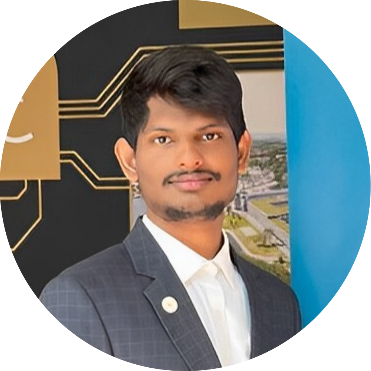
\includegraphics[width=2.7cm,clip]{images/resume_pic_m.png}
}
\parbox{\dimexpr\linewidth-3.8cm\relax}{
\vspace{-20pt}
\begin{tabularx}{\linewidth}{L r} \\
    {\Huge \scshape  Venkata Sai Yakkshit Reddy Asodi}~
    \href{https://www.cedzlabs.com/yakkshit}{\vspace{1pt}}\\
      Berlin, Germany. \\ \vspace{1pt}
     \small \raisebox{-0.1\height}\faPhone\ +91 8179936156 ~ \href{mailto:saiyakkshit2001@gmail.com}{\raisebox{-0.2\height}\faEnvelope\  {saiyakkshit2001@gmail.com}} ~ 
    \href{https://linkedin.com/in/yakkshit/}{\raisebox{-0.2\height}\faLinkedin\ {yakkshit}}  ~
    \href{https://yakkshit.com/}{\raisebox{-0.2\height}\faGlobe\ {yakkshit.com}}  ~
    \href{https://github.com/yakkshit}{\raisebox{-0.2\height}\faGithub{ yakkshit}}
    \vspace{-8pt}
\end{tabularx}
}
\end{center}
\vspace{-20pt}
\section{Summary}
Software Developer with 4+ years of experience specializing in Python, JavaScript, and TypeScript. Strong background in full-stack development, creating scalable applications using React and Django. Experienced in building AI-powered tools and working with large-scale visualizations. Adept at collaborating with cross-functional teams and optimizing frontend and backend solutions for efficient, secure, and user-friendly experiences.
\vspace{-10pt}

\section{Technical Skills}
\begin{itemize}[leftmargin=0.15in, label={}]
\small{\item{
\textbf{Languages: }{Python, JavaScript, TypeScript, HTML5, CSS3, SQL} \\
\textbf{Frameworks: }{React, Next.js, Django, Flask, Node.js} \\
\textbf{Tools: }{Docker, AWS, Kubernetes, Git, Postman, Swagger, Linux} \\
\textbf{Other: }{Machine Learning (TensorFlow, PyTorch), REST APIs, CI/CD pipelines}
}}
\end{itemize}
\vspace{-10pt}

\section{Experience}

\resumeSubHeadingListStart

\resumeSubheading
{Circleup AG}{January 2024 -- Present}
{Lead Full Stack Engineer (Frontend Focus)}{Zurich, Switzerland}
\begin{itemize}
\item Developed responsive web applications using React and Django, integrating APIs for AI-driven services.
\item Led the frontend design for AI diagnostic tools, focusing on large-scale image visualizations and data handling.
\item Collaborated with backend developers and machine learning teams to optimize API interactions for efficient data processing.
\end{itemize}
\vspace{-10pt}

\textbf{Full Stack Developer} \hfill Cedzlabs \\
\textit{Mar 2023 -- Jul 2024, India} 
\begin{itemize}
\item Built and maintained scalable web applications using React and Node.js for various AI-powered platforms.
\item Created user-friendly UIs with a focus on performance, accessibility, and cross-platform compatibility.
\end{itemize}
\vspace{-10pt}

\section{Projects}
\textbf{AI-Powered Pathology Visualization Tool} \\
\textit{Technologies: React, Django, Python, TensorFlow, Docker} 
\begin{itemize}
\item Designed and developed a web application for visualizing and annotating large-scale medical images for cancer diagnostics.
\item Implemented AI-powered features that analyze and highlight key areas in pathology slides, improving diagnostic accuracy.
\end{itemize}
\vspace{-5pt}

\textbf{AI Resume Generator} \\
\textit{Technologies: Next.js, Azure, LLMs, React} 
\begin{itemize}
\item Developed a resume generator using AI models to tailor resumes based on job descriptions, optimizing for specific roles and industries.
\item Deployed backend on Azure with secure data handling and fast performance.
\end{itemize}
\vspace{-5pt}

\section{Achievements}
\begin{itemize}
\item Developed machine learning tools to optimize data annotation pipelines, improving efficiency by 30\%.
\item Implemented CI/CD pipelines and Docker-based environments for seamless deployment and scalability.
\item Contributed to open-source projects focused on AI and full-stack development.
\end{itemize}
\vspace{-5pt}

\section{Languages}
\begin{itemize}
  \item English - Fluent $|$ German - Elementary $|$ Hindi - Fluent $|$ Telugu - Native
\end{itemize}

\end{document}